\documentclass{rvcepaper}
\begin{document}

% ---------- HS261TA Principles of Management and Economics
\begin{iempaper}
\paperinfo{dept={INDUSTRIAL ENGINEERING \& MANAGEMENT},date={4\textsuperscript{th} June 2025},exam={CIE -- II},maxmarks={10 + 50},sem={VI},prog={UG},duration={30 + 90 Min},code={}}
\begin{center}{\fontsize{12}{14}\selectfont DEPARTMENT OF}\\[3pt]{\bfseries\fontsize{15.5}{18}\selectfont INDUSTRIAL ENGINEERING \& MANAGEMENT}\end{center}\vspace{-3pt}
\noindent\begingroup\renewcommand{\arraystretch}{2.0}\bfseries\fontsize{11.5}{13}\selectfont
\begin{tabular}{|p{6.2cm}|C{5.0cm}|p{5.5cm}|}\hline
 Date \hspace{0.5cm}: \hspace{0.2cm}4\textsuperscript{th} June 2025 & CIE -- II & Max. Marks \hspace{0.3cm}: \hspace{0.2cm}10 + 50\\\hline
 Semester \hspace{0.1cm}: \hspace{0.2cm}VI & UG & Duration \hspace{0.55cm}: \hspace{0.2cm}30 + 90 Min\\\hline
 \multicolumn{3}{|C{16.7cm}|}{Principles of Management and Economics - HS261TA}\\\hline
\end{tabular}\endgroup\par\vspace{4pt}
\iemnote
\begin{cietable}{M}{BT}{CO}
\qpart{Part -- A}
\q{1.}{Differentiate between strategic goals and operational goals.}{02}{2}{2}
\q{2.}{In the BCG matrix, what does a ``Cash Cow'' represent?}{02}{2}{2}
\q{3.}{List any two types of corporate strategies and provide examples.}{02}{1}{2}
\q{4.}{How does an organic structure differ from a mechanistic structure?}{02}{2}{2}
\q{5.}{If the price elasticity of demand for a product is -0.5 and the price elasticity of supply is +2.5, what do these values imply about consumer and producer responses to price changes?}{02}{2}{4}
\qpart{Part -- B}
\q{1.}{Explain the strategic management process. Discuss each stage briefly and explain how this process helps organizations achieve their long-term objectives.}{10}{3}{2}
\q{2.}{A new entrant in the online grocery market wants to survive among large players like Amazon Fresh and BigBasket.
\begin{abc}
\item Use Porter's Five Forces to analyze the challenges.
\item Suggest a competitive strategy the company should adopt and why.
\end{abc}}{10}{4}{2}
\q{3.}{A growing bakery business is expanding from one shop to five locations. The owner notices confusion among staff regarding their tasks, delays in decision-making, and poor coordination between branches.
\begin{abc}
\item Explain the key elements of organizational structure.
\item For each element, suggest practical changes the company can implement to resolve the issues the bakery. Explain how these changes will improve organizational effectiveness.
\end{abc}}{10}{3}{2}
\q{4.}{Explain the concepts of demand and supply using appropriate diagrams. How is equilibrium price and quantity determined in a competitive market? What happens when there is a shift in either demand or supply?}{10}{2}{4}
\q{5.}{Two segments of the food delivery market are being studied:
\begin{bul}
\item Segment A includes dozens of local restaurants offering similar menus but trying to stand out through branding, discounts, and customer experience.
\item Segment B includes just three major food delivery platforms that dominate logistics, pricing control, and customer data.
\end{bul}
\textbf{Questions:}
\begin{abc}
\item Identify which segment represents \textbf{monopolistic competition} and which represents \textbf{oligopoly}, justifying your answer with characteristics of each market structure.
\item Compare and contrast the pricing strategies and customer acquisition methods used in both segments.
\item As a new entrepreneur entering the market, which segment would you prefer to compete in and why? Base your answer on market behavior, barriers to entry, and strategic flexibility.
\end{abc}}{10}{4}{4}
\end{cietable}
\end{iempaper}

% ---------- IM362IA Supply Chain Management
\begin{iempaper}
\paperinfo{shownote=0,date={06.05.2025},exam={CIE -- II},maxmarks={10 + 50},sem={VI},prog={UG},duration={30 + 90 Min},
 title={Supply Chain Management},code={IM362IA}}
\iemhead
{\small Note:}\par\vspace{-1pt}
\hspace*{0.5cm}{\footnotesize 1. \hspace{0.1cm}Answer all the Questions.}\par
\hspace*{0.5cm}{\footnotesize 2. \hspace{0.1cm}Use of Normal Distribution Tables permitted.}\par\vspace{3pt}
\begin{cietable}{M}{BT}{CO}
\qpart{Part -- A}
\q{1.}{\begin{minipage}[t]{3.4cm}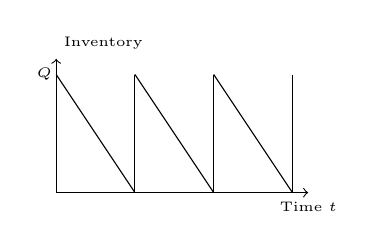
\begin{tikzpicture}[x=0.5cm,y=0.5cm,font=\tiny]
\draw[->] (0,0) -- (0,3.4) node[above,xshift=0.6cm] {Inventory}; \draw[->] (0,0) -- (6.4,0) node[below] {Time $t$};
\draw (0,3) -- (2,0); \draw (2,3) -- (4,0); \draw (4,3) -- (6,0); \draw (0,3) -- (0,0); \draw (2,3) -- (2,0); \draw (4,3) -- (4,0); \draw (6,3) -- (6,0);
\node at (-0.3,3) {$Q$};
\end{tikzpicture}\end{minipage}\hspace{1.2cm}\begin{minipage}[t]{5cm}What is the inference drawn from the figure?\end{minipage}}{2}{1}{CO3}
\q{2.}{The primary role of cycle inventory is to allow different stages in the supply chain to purchase product in lot sizes that minimize the sum of the \blank[3.2cm], \blank[1.9cm], and \blank[1.9cm] cost.}{2}{1}{CO3}
\q{3.}{A key to reducing lot size without \blank[2.4cm] costs is to \blank[2.4cm] the fixed cost associated with each lot.}{2}{1}{CO3}
\q{4.}{List the Macro-economic factors influencing network design decisions.}{2}{1}{CO2}
\q{5.}{Illustrate different flexibility configurations in network.}{2}{1}{CO2}
\qpart{Part --B}
\q{1}{Develop the framework for network design decisions. Analyze the various phases.}{10}{3}{CO2}
\q{2}{Explain the methodology of evaluating network design decisions using decision trees.}{10}{3}{CO2}
\q{3}{Demand for the Deskpro computer at Best Buy is 1,000 units per month. Best Buy incurs a fixed order placement, transportation, and receiving cost of \$4,000 each time an order is placed. Each computer costs Best Buy \$500 and the retailer has a holding cost of 20 percent. Evaluate the number of computers that the store manager should order in each replenishment lot, number of orders per year, annual inventory cost, and average flow time.}{10}{3}{CO3}
\q{4}{Write a detailed note on multi-echelon cycle inventory.}{10}{2}{CO3}
\q{5 a.}{Assume that weekly demand for phones at B\&M Office Supplies is normally distributed, with a mean of 2,500 and a standard deviation of 500. The manufacturer takes two weeks to fill an order placed by the B\&M manager. The store manager currently orders 10,000 phones when the inventory on hand drops to 6,000. Evaluate the safety inventory and the average inventory carried by B\&M. Also evaluate the average time a phone spends at B\&M.}{05}{4}{CO3}
\q{5 b.}{Weekly demand for Legos at a Wal-Mart store is normally distributed, with a mean of 2,500 boxes and a standard deviation of 500. The replenishment lead time is two weeks. Assuming a continuous review replenishment policy, evaluate the safety inventory that the store should carry to achieve a CSL of 90 percent.}{05}{}{}
\end{cietable}
\end{iempaper}

% ---------- IM363IA Ergonomics
\begin{iempaper}
\paperinfo{date={9\textsuperscript{th} June 2025},exam={CIE -- 2},maxmarks={10 + 50},sem={VI},prog={UG},duration={30 + 90 Min},
 title={ERGONOMICS},code={IM363IA}}
\iemhead
\begin{cietable}{M}{BT}{CO}
\qpart{Part -- A}
\q{1.}{Which type of control is most suited for precise positioning tasks?}{01}{L$_2$}{CO1}
\q{2.}{What is the principle of ``legibility'' in display design?}{01}{L$_1$}{CO2}
\q{3.}{What ergonomic principle recommends grouping related controls together?}{01}{L$_2$}{CO2}
\q{4.}{Give one example, on how you utilize the concept of minimizing information access cost to ATM screen design.}{01}{L$_3$}{CO1}
\q{5.}{State where a desktop monitor should be positioned for ergonomic efficiency based on anthropometric data.}{01}{L$_2$}{CO2}
\q{6.}{State how the redundancy gain principle is used in designing emergency alerts.}{01}{L.2}{CO2}
\q{7.}{What is the primary ergonomic concern in designing for children?}{01}{L$_2$}{CO2}
\q{8.}{Give one example of assistive technology.}{01}{L$_1$}{CO1}
\q{9.}{What is one reason to avoid ``one-size-fits-all'' designs?}{01}{L$_2$}{CO2}
\q{10.}{Name one cognitive difference relevant in the design for children.}{01}{L$_1$}{CO1}
\qpart{Part -- B}
\q{1.}{Explain how you would apply the Principles of Display Design when designing a monitoring panel in an industrial plant.}{10}{L$_3$}{CO2}
\q{2.}{Compare and contrast discrete and continuous controls in terms of their ergonomic applicability with suitable examples.}{10}{L$_3$}{CO2}
\q{3 a.}{Briefly outline how the principles of Fitts's Law is applied to justify the optimal placement of frequently used touch controls on a tablet interface.}{05}{L$_3$}{CO3}
\q{b.}{A user navigates to a target 160 mm away and 40 mm wide. With a = 80 and b = 90, compute movement time.}{05}{L$_3$}{CO2}
\q{4.}{How can anthropometric data be used to improve the user interface of a digital product? Provide examples involving touchscreens, workstations, or ATMs.}{10}{L$_3$}{CO2}
\q{5.}{Discuss the special considerations to be taken into account when designing for children. Highlight how anthropometric data of children differs from that of adults.}{10}{L$_4$}{CO4}
\end{cietable}
\end{iempaper}

% ---------- IM365TDA Facilities Planning and Design
\begin{iempaper}
\paperinfo{shownote=0,date={6\textsuperscript{th} June 2025},exam={CIE -- 2},maxmarks={10 + 50},sem={VI},prog={UG},duration={30 + 90 Min},
 title={FACILITIES PLANNING AND DESIGN},code={IM365TDA}}
\iemhead
{\small Note: Answer all the Questions.}\par\vspace{3pt}
\ptitle{PART A}
\begin{longtable}{|C{1.3cm}|p{11.95cm}|C{0.95cm}|C{0.95cm}|C{0.95cm}|}
\hline \textbf{Q No.1} & \multicolumn{1}{c|}{\textbf{Questions}} & \textbf{M} & \textbf{BT} & \textbf{CO}\\\hline
\q{1.1}{Given station times:
\begin{bul}\item Station 1: 5 min \item Station 2: 4 min \item Station 3: 6 min\end{bul}
Find the bottleneck.}{01}{2}{1}
\q{1.2}{Total task time = 20 minutes, Number of workstations = 4, Cycle time = 6 minutes\newline Find line efficiency.}{02}{1}{1}
\q{1.3}{Calculate Throughput Time. Given:
\begin{bul}\item Station A: 2 min \item Station B: 3 min \item Station C: 4 min\end{bul}
What is the total throughput time for one product?}{02}{2}{1}
\q{1.4}{If a production unit has limited floor space and needs to allow a single operator to handle multiple machines easily, which layout (S-flow or U-flow) is better?}{01}{1}{1}
\q{1.5}{Define a unit load as per Tanchoco et al.}{02}{2}{1}
\q{1.6}{List any two basic methods of moving the unit load according to Apple.}{01}{1}{1}
\end{longtable}
\ptitle{Part --B}
\begin{cietable}{M}{BT}{CO}
\q{1}{State and explain the different types of material flow with suitable examples.}{10}{2}{1}
\q{2}{A factory is designing a new assembly line for producing electric scooters. The production involves 5 sequential tasks with the following task times (in minutes):
\qtab{|c|c|}{\hline Task & Time (min)\\\hline A & 4\\\hline B & 6\\\hline C & 5\\\hline D & 3\\\hline E & 2\\\hline}
The management is considering either a Straight Line Flow layout or a U-Flow layout. Tasks:\newline
a) Calculate the total time required to complete one unit.\newline
b) Identify the bottleneck in the process.\newline
c) If the total cycle time is 6 minutes and there are 3 workstations, compute the line efficiency.\newline
d) Which layout (S-Flow or U-Flow) would you recommend if space is limited and one operator needs to handle multiple stations? Justify your answer}{10}{3}{3}
\q{3}{What are the Factors for Consideration in Planning Material Flow}{10}{2}{2}
\q{4}{Enumerate and elaborate the steps in material handling system design.}{10}{1}{2}
\q{5}{Explain the guidelines for estimating the material handling costs in practice.}{10}{1}{1}
\end{cietable}
\end{iempaper}

% ---------- IM365TDB Service Operations Management
\begin{iempaper}
\paperinfo{date={6-6-2025},exam={CIE -- 2},maxmarks={10 + 50},sem={VI},prog={UG},duration={30 + 90 Min},
 title={Service Operations Management},code={IM365TDB}}
\iemhead
\begin{cietable}{M}{BT}{CO}
\qpart{Part -- A}
\q{1.}{Think of a time when you recently received poor service. If service operations are so important, identify reasons why poor service is delivered sometimes?}{2}{2}{1}
\q{2.}{Assume you get in to an ``IT enabled service'' (ITES) industry in the next five years. Comment on how you intend to use Service as a competitive advantage.}{2}{4}{3}
\q{3.}{What is the service concept of ``Cyber nurseries''.}{2}{2}{2}
\q{4.}{Comment on the importance of service process design.}{2}{3}{4}
\q{5.}{From your experience, give two examples where technology is used to enhance customer experience.}{2}{2}{2}
\qpart{Part -- B}
\q{1}{Discuss the role of technology in developing the customer Experience. Cite two examples of services where technology has been used effectively to enhance customer experience.}{10}{3}{4}
\q{2}{The nature of supply chains can be very messy and complex. Describe the key issues service operations managers should focus on with a key focus on managing through intermediaries.}{10}{3}{4}
\q{3}{Write short notes on
\begin{abc}\item Service level agreements (SLA)\item Difference between SLA and Operational Level Agreements (OLA)\end{abc}}{10}{2}{3}
\q{4}{Visualize an experience map for a customer visiting a typical dental clinic.}{10}{4}{2}
\q{5}{One of the key decisions for procurement function is choosing/selecting a supply partner and particularly for those who handle critical elements of supply chain. Discuss the criteria for supplier selection excluding Cost and Quality.}{10}{4}{4}
\end{cietable}
\end{iempaper}

% ---------- IM364TA Human Resource Management & Analytics
\begin{iempaper}
\paperinfo{code={}}
\begin{center}{\fontsize{12}{14}\selectfont DEPARTMENT OF}\\[3pt]{\bfseries\fontsize{15.5}{18}\selectfont INDUSTRIAL ENGINEERING \& MANAGEMENT}\end{center}\vspace{-3pt}
\noindent\begingroup\renewcommand{\arraystretch}{2.0}\bfseries\fontsize{11.5}{13}\selectfont
\begin{tabular}{|p{6.2cm}|C{5.0cm}|p{5.5cm}|}\hline
 Date \hspace{0.5cm}: \hspace{0.2cm}5\textsuperscript{th} June 2025 & CIE -- II & Max. Marks \hspace{0.3cm}: \hspace{0.2cm}10 + 50\\\hline
 Semester \hspace{0.1cm}: \hspace{0.2cm}VI & UG & Duration \hspace{0.55cm}: \hspace{0.2cm}30 + 90 Min\\\hline
 \multicolumn{3}{|C{16.7cm}|}{Human Resource Management \& Analytics - IM364TA}\\\hline
\end{tabular}\endgroup\par\vspace{4pt}
\iemnote
\begin{cietable}{M}{BT}{CO}
\qpart{Part -- A}
\q{1.}{Differentiate between content validity and criterion validity in test.}{02}{L1}{CO2}
\q{2.}{Define unstructured interview and structured interview.}{02}{L2}{CO2}
\q{3.}{Mention the ways to evaluate training effectiveness.}{02}{L2}{CO3}
\q{4.}{Define behaviorally anchored rating scale.}{02}{L1}{CO3}
\q{5.}{Explain reactive decision-making and predictive decision-making in HR.}{02}{L2}{CO3}
\qpart{Part -- B}
\q{1.}{Elaborate on the major types of employment selection tests that organizations use during recruitment. For each category, describe its purpose, what it measures, and provide relevant job-related examples to illustrate its application in real-world hiring.}{10}{L2}{CO2}
\q{2.}{Describe the different types of interviews used in the selection process with examples and how does theses interview types help assess candidate suitability.}{10}{L3}{CO2}
\q{3.}{Imagine you are responsible for implementing a training program. Outline the systematic steps involved in designing and executing an effective training process. For each step, explain its role and importance in ensuring the training meets both organizational and employee development goals.}{10}{L3}{CO3}
\q{4.}{Identify frequent challenges or errors that reduce the effectiveness of performance appraisals. Suggest strategies or best practices that can be adopted to minimize these issues and improve the overall fairness, accuracy, and impact of the appraisal system.}{10}{L2}{CO3}
\q{5.}{Describe the framework of HR Analytics. Discuss the key components and explain how they contribute to strategic HR decision-making.}{10}{L2}{CO3}
\end{cietable}
\stars{----*****----}
\end{iempaper}

% ---------- AS266TEA Fundamentals of Aerospace Engineering
\begin{xpaper}
\paperinfo{deptline={Department of Aerospace Engineering},date={06/06/25},exam={Test - 2},maxmarks={60},sem={VI},prog={UG},duration={$1\frac{1}{2}$ Hrs},
 title={Fundamentals of Aerospace Engineering},code={AS266TEA}}
\xhead
\begin{xtable}{Questions}
\q{1}{Among the various gas turbine engine derivatives, \blank[1.8cm] engine has the lightest specific weight.}{01}{L1}{1}
\q{2}{Achieving thrust reversals is quite easy in case of \blank[1.8cm] engines.}{01}{L2}{2}
\q{3}{\blank[1.8cm] aids in decreasing the speed and increasing the torque of the propeller shaft connecting the propeller and the turbine of the engine.}{01}{L2}{3}
\q{4}{Fluid Friction is one of the major factors contributing towards the increase of \blank[1.8cm] in an Ideal Brayton cycle.}{01}{SL2}{2}
\q{5}{\blank[1.8cm] is an aerodynamic force acting perpendicular to the chord of a cambered airfoil.}{01}{L3}{2}
\q{6}{\blank[1.8cm] is defined as the location on an airfoil where the distribution of forces results in zero moment.}{01}{L2}{1}
\q{7}{To get additional lift during take-off, the pilot needs to deploy \blank[1.8cm] of an airplane.}{01}{L2}{2}
\q{8}{Define aerodynamic center of a wing.}{01}{L2}{4}
\q{9}{What is meant by by-pass ratio of a turbofan engine.}{01}{L2}{4}
\q{10}{List the various types of drag experienced by a airplane in flight.}{01}{L2}{3}
\qpart{PART B}
\q{1}{Depicting the various components of a pure turbojet engine on neat sketch, explain its working principle. Also, list the advantages and disadvantages of the turbojet engine.}{10}{L1}{CO2}
\q{2}{Illustrating a neat sketch of a gas turbine engine, explain the operation of Brayton cycle.}{10}{L3}{CO3}
\q{3}{Define stalling. With a neat sketch, explain the physical phenomenon of the occurrence of stall with respect to the airfoils angle of attack.}{10}{L2}{CO2}
\q{4}{An aircraft has an effective wing area of 78m\textsuperscript{2}. It is in level flight at a speed of 750km/h at an altitude where the density is 0.467kg/m\textsuperscript{3}. If the weight of the aircraft is 495kN. Find the coefficient of lift for the wing section. If the coefficient of drag is 10\% of the C\textsubscript{L}. Determine the thrust required for level flight.}{10}{L3}{CO4}
\q{5}{Draw a neat diagram of a typical wing planform geometry. Highlight all the parts of the wing and explain.}{10}{L3}{CO3}
\end{xtable}
\end{xpaper}

% ---------- BT266TEB Healthcare Analytics (Test - 2)
\begin{iempaperB}
\paperinfo{ayear={2024-2025 (Even Sem)},usn=0,rule=0,dept={BIOTECHNOLOGY},date={June, 2025},code={BT266TEB},sem={VI Semester},exam={Closed Book Offline Quiz and Test -- 2},maxmarks={10 + 50},duration={120 min},
 title={Healthcare Analytics (Institutional Elective)},shownote=0}
\vspace{-0.2cm}\centerline{Common to all branches}\par
\iemheadB
{\small Answer all questions in Part A \& Part B, Answer Part A in first two pages in sequence only}\par\vspace{2pt}
\ptitle{Part A}
\begin{xtable}{Questions}
\q{1}{Multiple sequence analysis consists \blank[2cm] or more number of sequences.}{1}{2}{1}
\q{2}{Needleman\_Wunsch algorithm can be applied for \blank[2cm] alignment.}{1}{2}{1}
\q{3}{A phylogenetic tree represents \blank[2cm]}{1}{2}{2}
\q{4}{Among the PAM1 and PAM250, which one has the more distant?}{1}{3}{2}
\q{5}{Differentiate between the opening and extension gap penalties.}{2}{2}{3}
\q{6}{What is null hypothesis?}{2}{4}{3}
\q{7}{Mention any 2 measures of statistical significance.}{2}{2}{4}
\end{xtable}
\ptitle{Part B}
\begin{xtable}{Questions (Test)}
\q{1.}{Illustrate on the various types of sequence alignments. Explain any one in brief.}{10}{2}{3}
\q{2}{How does the scoring matrix helps to derive the interpretation among sequence alignment?}{10}{3}{3}
\q{3}{Elucidate on the profiles and Hidden Morkov Models for bioinformatics data.}{10}{4}{4}
\q{4}{Differentiate between PAM and BLOSSUM and write its significance.}{10}{4}{4}
\q{5}{Write an overview of molecular phylogeny.}{10}{2}{3}
\end{xtable}
\btfoot{|l|l|l|*{10}{C{0.9cm}|}}{\hline
\multirow{2}{*}{Marks Distribution} & Particulars & & CO1 & CO2 & CO3 & CO4 & L1 & L2 & L3 & L4 & L5 & L6\\\cline{2-13}
 & Test & Max Marks & & & 60 & 40 & & 40 & 20 & 40 & & \\\hline}
\end{iempaperB}

% ---------- CH266TEC Industrial Safety Engineering (Test - 2)
\begin{xpaper}
\paperinfo{deptline={Department of Chemical Engineering},date={04.06.2025},exam={Test - 2},maxmarks={60},sem={6},prog={UG},duration={2 Hrs},
 title={Industrial Safety Engineering},code={CH266TEC}}
\xhead
\begin{xtable}{Questions}
\q{1}{What is the certainty coefficient if cash outflow to a project is 100000 and certain cash flow is 50000?}{02}{03}{02}
\q{2}{Determine Severity Rate with two recordable injuries, if an employee breaks leg on a Monday, and loses the rest of that day plus three additional days of work, then the employee comes back to work the following Friday and is given restricted work tasks, and then loses another two days.}{02}{03}{02}
\q{3}{Expand RADR and OIR}{02}{02}{02}
\q{4}{Write process hazard worksheet table that is used in PHA analysis.}{02}{02}{2}
\q{5}{Write Fault tree event symbols for basic event and underdeveloped event.}{02}{02}{2}
\qpart{PART B}
\q{1}{What is Fault Tree? Construct the Fault and Event trees for the process consist of reactor system with heating and cooling arrangement to maintain constant reactor temperature.}{10}{03}{03}
\q{2}{What is Preliminary hazard analysis? Classify and explain preliminary hazard analysis table for FMEA, HAZOP and operator related hazards.}{10}{02}{02}
\q{3}{Draw a flowchart and explain the basic concept of Safety Domain Ontology.}{10}{01}{03}
\q{4}{A project is required to invest INR. 1,10,000 and is expected to generate cash flow after tax over its economic life time of 5 years of INR 20,000, INR30,000, INR35,000, INR 55,000 and INR 10,000. Risk free interest rate is 7 per cent and decision maker interested to add 3 per cent as risk premium for the project. Calculate NPV using RADR approach and suggest on the acceptability of the project.}{05}{03}{03}
\q{5}{The following are the possible net cash flows of Project X and Y and their associated probabilities. Both projects have a discount rate 10 per cent. Calculate the expected NPV for each project if initial investment in both cases is 5000. Calculate variance, standard deviation and coefficient of variation and comment which project is preferable?}{15}{03}{04}
\end{xtable}
\end{xpaper}

% ---------- CS266TED Robotic Process Automation (Test - 2)
\begin{xpaper}
\paperinfo{deptline={Department of Computer Science and Engineering},date={June 2025},exam={Test - 2},maxmarks={60},sem={VI},prog={UG},duration={2 Hrs},
 title={ROBOTIC PROCESS AUTOMATION},code={CS266TED}}
\xhead
\ptitle{PART A}
\begin{xtable}{Questions}
\q{1.}{List the actions that cannot be recorded in UiPath}{02}{2}{1}
\q{2.}{What is an UI element?}{01}{2}{1}
\q{3.}{To extract information from virtual environment \blank[2cm] output method is used}{01}{1}{1}
\q{4.}{Define data scraping.}{01}{1}{2}
\q{5.}{What is relative scraping? How does it work?}{02}{2}{1}
\q{6.}{Outline different types of user interfaces in UiPath.}{02}{2}{2}
\q{7.}{\blank[2cm] activity is used to extract data from the DataTable.}{01}{1}{1}
\end{xtable}
\ptitle{PART B}
\begin{xtable}{Questions}
\q{1. a}{Discuss different types of recorders in UiPath. Explain any two.}{06}{2}{2}
\q{b}{Describe copy activity of the recorder in UiPath.}{04}{3}{2}
\q{2. a}{List the various input methods supported in UiPath and discuss the key differences between them.}{06}{2}{3}
\q{b}{Identify the steps of data scraping wizard.}{04}{3}{3}
\q{3. a}{Describe in detail OCR output method provided in UiPath.}{04}{3}{3}
\q{b}{Explain various activities related to Data Scraping.}{06}{3}{2}
\q{4. a}{Elaborate on various types of selectors available in UiPath.}{04}{2}{2}
\q{b}{Analyse the usage of the UI Explorer with an appropriate example.}{06}{3}{2}
\q{5. a}{Name and explain the processes involved in Retrieving Information.}{04}{4}{3}
\q{b}{What are anchors? Describe its usage in PDF documents with a workflow.}{06}{4}{4}
\end{xtable}
\cotable{\textbf{Course Outcomes}}{CO1 & Understand RPA principles, its features and applications\\\hline CO2 & Demonstrate proficiency in handling variables and decision making inside a workflow and data manipulation techniques.\\\hline CO3 & Gain insights into recording, email automation and exception handling and orchestrator\\\hline CO4 & Analyze the trends in automation and choose business strategy to design a real world automation workflow.}
\btfoot{|l|*{6}{C{1.1cm}|}*{5}{C{1.2cm}|}}{\hline BT \& CO Marks & L1 & L2 & L3 & L4 & L5 & L6 & CO1 & CO2 & CO3 & CO4 & CO5\\\hline & 3 & 23 & 24 & 10 & -- & -- & 7 & 33 & 14 & 6 & --\\\hline}
\end{xpaper}

% ---------- CV266TEE Intelligent Transportation System (CIE - 2)
\begin{xpaper}
\paperinfo{deptline={Department of Civil Engineering},date={},exam={CIE - 2},maxmarks={60},sem={VI},prog={UG},duration={2 Hrs},
 title={Intelligent Transportation System},code={CV266TEE}}
\xhead
\ptitle{Quiz}
\begin{xtable}{Questions}
\q{1.}{List any two functionalities required for ITS user services.}{2}{2}{1}
\q{2.}{Mention two methods of data acquisition in ITS.}{2}{2}{1}
\q{3.}{Explain the importance of ITS physical architecture.}{2}{2}{2}
\q{4.}{Mention any two technology building blocks of ITS.}{2}{2}{1}
\q{5.}{Describe the role of communication tools in ITS.}{2}{2}{2}
\end{xtable}
\ptitle{Test}
\begin{xtable}{Questions}
\q{1.}{Analyze the differences between logical and physical ITS architectures.}{10}{2}{1}
\q{2.}{Analyze the roles of detection, identification, and collection methods in ITS performance.}{10}{3}{1}
\q{3.}{Examine the contribution of each ITS building block in improving urban transportation efficiency.}{10}{2}{1}
\q{4.}{Discuss the importance and limitations of ITS standards in national implementations.}{10}{3}{2}
\q{5.}{Propose a detailed ITS evaluation framework for a newly implemented smart city transport project.}{10}{5}{2}
\end{xtable}
\end{xpaper}

% ---------- CM266TEG Advanced Energy Storage for E-Mobility (Test - 2)
\begin{xpaper}
\paperinfo{deptline={Department of Chemistry},date={04-06-2025},exam={Test - 2},maxmarks={50},sem={6},prog={UG},duration={$1\frac{1}{2}$ Hrs},
 title={ADVANCED ENERGY STORAGE FOR E-MOBILITY},code={CM266TEG}}
\xhead
\begin{xtable}{Questions}
\q{1}{Apply your understanding of sodium-based battery chemistries to explain different types of sodium batteries. Using a neat and labelled diagram, describe the construction and working of a sodium-sulfur (Na-S) battery along with advantages in safety point of view.}{10}{3}{4}
\q{2}{Outline the construction and working of advanced lead acid battery along with chemical reactions involved during charging and discharging. Mention its advantages.}{10}{2}{1}
\q{3}{Compare the electrochemical performance of lithium iron phosphate (LFP) with that of lithium cobalt oxide battery. Explain the working mechanism of Lithium iron phosphate battery along with neat labelled diagram.}{10}{4}{3}
\q{4}{Illustrate the construction and working of lithium-sulfur batteries and discuss their advantages and limitations. Comment on the polysulfide shuttle mechanism in such type of battery.}{10}{3}{2}
\q{5}{Explain how the ZEBRA (Sodium Nickel Chloride) battery operates and its suitability for commercial applications. Discuss the advantages and limitations of zebra battery.}{10}{2}{1}
\end{xtable}
\end{xpaper}

% ---------- CM266TEG Advanced Energy Storage for E-Mobility (Quiz - 2)
\begin{xpaper}
\paperinfo{deptline={Department of Chemistry},date={04-06-2025},exam={Quiz - 2},maxmarks={10},sem={6},prog={UG},duration={$\frac{1}{2}$ Hrs},
 title={ADVANCED ENERGY STORAGE FOR E-MOBILITY},code={CM266TEG}}
\xhead
\begin{xtable}{Questions}
\q{1}{Give an example for the cathode materials used in lithium sulphur battery.}{1}{1}{}
\q{2}{Identify one difference between sodium-ion and lithium-ion batteries.}{1}{2}{}
\q{3}{Name the electrolyte used in lithium-sulphur batteries.}{1}{2}{}
\q{4}{Illustrate with one example how a battery's chemistry affects charging speed.}{1}{3}{}
\q{5}{Name the material which deposits during charging and discharging of lead acid battery.}{1}{1}{}
\q{6}{Lithium battery has very high capacity than that of lead acid battery. justify}{1}{5}{}
\q{7}{Justify why sodium-sulphur batteries are not commonly used in consumer electronics.}{1}{5}{}
\q{8}{Suggest an appropriate non-lithium battery for grid storage applications.}{1}{3}{2}
\q{9}{Analyse the main limitation of lithium-air batteries in practical applications.}{1}{5}{4}
\q{10}{Apply your knowledge to name one battery suitable for low-temperature EV operations.}{1}{3}{2}
\end{xtable}
\end{xpaper}

% ---------- EC266TEH Human Machine Interface (Test - 2 + Quiz - II)
\begin{xpaper}
\paperinfo{deptline={Department of Electronics and Communication Engineering},date={4.6.2025},exam={Test - 2},maxmarks={50},sem={VI},prog={UG},duration={$1\frac{1}{2}$ Hrs $+\frac{1}{2}$ Hrs},
 title={Human Machine Interface},code={EC266TEH}}
\xhead
\begin{xtable}{Questions}
\q{1.a.}{List any FOUR differences between UX and UI.}{4}{1}{1}
\q{1.b.}{Discuss the core components of UX designing applications.}{6}{2}{1}
\q{2.a.}{Explain the advantageous of Mobile HMI for industrial applications.}{4}{2}{1}
\q{2.b.}{List and explain the 5 elements of UX in detail with neat diagrams.}{6}{2}{2}
\q{3.a.}{Discuss the key roles of web server in HMI Application.}{5}{2}{2}
\q{3.b.}{List the main stages of the user-cantered HMI development process and explain the importance of each stage.}{5}{2}{2}
\q{4.a.}{Illustrate the Design Thinking process in detail for HMI applications.}{6}{2}{3}
\q{4.b.}{Explain five common User Experience asset design types.}{4}{2}{1}
\q{5.a.}{Discuss the 5 Dimensions of Interactive design used for SCADA Applications.}{5}{2}{2}
\q{5.b.}{What is a web server? Describe in brief the main components of a web server.}{5}{1}{1}
\end{xtable}
\par\vspace{6pt}
\begin{xtable}{Quiz -II}
\q{1.}{Cross-platform application programming interface (API) for rendering 2D and 3D vector graphics is called \blank[2.4cm]}{1}{1}{1}
\q{2.}{The style and formatting of text used in a product, including font families, sizes, and weights is called \blank[2.4cm]}{1}{1}{1}
\q{3.}{Simple sketches or digital mockups that show the layout, structure, and organization of content on a webpage or app screen are called \blank[2.4cm]}{1}{1}{1}
\q{4.}{Fictional characters that represent the target users of a product, used to guide design decisions and keep the user's needs in mind are known as \blank[2.4cm]}{1}{1}{1}
\q{5.}{Name any 2 prototyping tools for UX.}{1}{1}{1}
\q{6.}{Name two accessibility features that should be considered in a mobile HMI.}{1}{2}{1}
\q{7.}{\blank[2.4cm] protocol is most commonly used for communication between a webserver and a browser-based HMI.}{1}{2}{1}
\q{8.}{Which of the following is considered a fundamental UI design component?}{1}{1}{2}
\q{9.}{\blank[2.4cm] file format is most commonly used for vector design assets.}{1}{1}{1}
\q{10.}{The main benefit of using vector assets in design \blank[2.4cm]}{1}{1}{1}
\end{xtable}
\end{xpaper}

% ---------- IM266TEQ Elements of Financial Management (CIE - II)
\begin{iempaper}
\paperinfo{shownote=0,date={4\textsuperscript{th} June 2025},exam={CIE-- II},maxmarks={10 + 50},sem={VI},prog={UG},duration={30 + 90 Min},
 title={Elements of Financial Management (Institutional Elective)},code={IM266TEQ}}
\iemhead
{\small Note:}\par\vspace{-1pt}
\hspace*{0.5cm}{\footnotesize 1. \hspace{0.1cm}Answer all the Questions.}\par
\hspace*{0.5cm}{\footnotesize 2. \hspace{0.1cm}Avoid verbose answers and answer specifically and to the point.}\par\vspace{3pt}
\begin{cietable}{M}{BT}{CO}
\qpart{Part -- A}
\q{1.}{List the three commonly used approaches employed for valuation of equities.}{02}{L3}{CO2}
\q{2.}{Distinguish between Market Risk and Unique Risk.}{02}{L2}{CO2}
\q{3.}{In the context of long- term financing, distinguish between Equity and Debt in terms of the ownership rights to the investor.}{02}{L2}{CO4}
\q{4.}{What does the term Yield to Maturity represent?}{01}{L2}{CO2}
\q{5.}{What does the term ``Risk'' in Finance primarily refer to?}{01}{L1}{CO3}
\q{6.}{Mention any one capital budgeting technique that considers the time value of money.}{01}{L1}{CO3}
\q{7.}{Name the capital budgeting technique that calculates profitability as a percentage of investments.}{01}{L1}{CO3}
\qpart{Part -- B}
\q{1 a.}{A bond with a face value of \rupee 1,000 carries a coupon rate of 10\% and matures in 5 years. If the required rate of return is 8\%, calculate the value of the bond.}{05}{L3}{2}
\q{b.}{A bond with a face value of \rupee 1,000 sells for \rupee 950. It has a 10\% annual coupon and matures in 5 years. Calculate the Yield to Maturity.}{05}{L3}{2}
\q{2 a.}{An investor is analysing a stock with the following possible returns and probabilities:
\qtabc{|c|c|c|}{\hline Scenario & Return (\%) & Probability\\\hline Boom & 20 & 0.3\\\hline Normal & 10 & 0.5\\\hline Recession & -5 & 0.2\\\hline}
Calculate the Expected Return and also the Standard Deviation of the returns.}{07}{L3}{2}
\q{b.}{Relationship between risk and Return is one of the fundamental Principles in Financial decisions in organizations. Justify}{03}{L2}{2}
\q{3.}{Enumerate the steps involved in Capital Budgeting Process.}{10}{L2}{3}
\q{4 a.}{There are two Projects for consideration. Apply Net Present Value method and determine the Project to be chosen.\newline
Project A: \rupee 20,000 investment, \rupee 6,000 for 5 years\newline
Project B: \rupee 20,000 investment, \rupee 10,000 for 2 years\newline
Rate = 10\%}{05}{L4}{3}
\q{b.}{A project costs \rupee 150,000 with no residual value. It yields accounting profits of \rupee 10,000, \rupee 12,000, \rupee 14,000, \rupee 16,000, and \rupee 18,000 over 5 years. Calculate Average Rate of Return and interpret.}{05}{L4}{3}
\q{5.}{Explain any Five sources of long term finance available to business organizations.}{10}{L2}{4}
\end{cietable}
\stars{******}
\end{iempaper}

% ---------- MA266TEU Mathematical Modelling (CIE - 2)
\begin{xpaper}
\paperinfo{deptline={Department of Mathematics},date={04/06/2025},exam={CIE - 2},maxmarks={100},sem={VI},prog={UG},duration={2 Hrs. (2pm-4pm)},
 title={Mathematical Modelling},code={MA266TEU}}
\xhead
\begin{longtable}{|C{1.05cm}|p{12.2cm}|C{0.95cm}|C{0.95cm}|C{0.95cm}|}
\hline \textbf{SL. No} & \multicolumn{1}{c|}{\textbf{Quiz: Questions}} & \textbf{M} & \textbf{BTL} & \textbf{CO}\\\hline
\q{1}{The Fibonacci Numbers 1, 1, 2, 3, 5, 8, 13, 21,\ldots can be modelled in a difference equation of the form \blank[2cm].}{2}{2}{2}
\q{2}{Solve $u_{t+1}=8x_t$, $x_0=\frac{1}{2}$.}{2}{1}{1}
\q{3}{With respect to a characteristic brown eyes, suppose the proportions of the dominants, hybrids and recessives in 9\textsuperscript{th} generation are $p_9$, $q_9$ and $r_9$ respectively, then $r_{10}=$ \blank[1.5cm], and $q_{10}=$ \blank[1.5cm].}{2}{1}{1}
\q{4}{In the long run, the proportion of time that the given Markov chain will be in state A is \blank[1.5cm] and state B is \blank[1.5cm].
\par\vspace{2pt}\centerline{\begin{tikzpicture}[>=Stealth,node distance=2.4cm,every node/.style={font=\small}]
\node[draw,circle,minimum size=0.7cm,inner sep=0] (A) at (0,0) {A}; \node[draw,circle,minimum size=0.7cm,inner sep=0] (B) at (2.8,0) {B};
\draw[->] (A) to[loop left] node[left] {0.3} (A); \draw[->] (B) to[loop right] node[right] {0.2} (B);
\draw[->] (A) to[bend left=25] node[above] {0.7} (B); \draw[->] (B) to[bend left=25] node[below] {0.8} (A);
\end{tikzpicture}}}{2}{3}{2}
\q{5}{Find the fixed probability vector of the stochastic matrix $A=\begin{bmatrix}3/4&1/4\\1/2&1/2\end{bmatrix}$.}{2}{3}{3}
\end{longtable}
\begin{longtable}{|C{1.05cm}|p{12.2cm}|C{0.95cm}|C{0.95cm}|C{0.95cm}|}
\hline \textbf{SL. No} & \multicolumn{1}{c|}{\textbf{Test}} & \textbf{M} & \textbf{BTL} & \textbf{CO}\\\hline
\q{1.}{Develop a model through difference equations in genetics based on Hardy-Weinberg law.}{10}{2}{2}
\q{2.}{Discuss Cobweb model about the variation of price and quantity of a commodity produced by a farm.}{10}{2}{2}
\q{3.}{Prove that the Markov chain with transition probability matrix $\begin{bmatrix}0&2/3&1/3\\1/2&0&1/2\\1/2&1/2&0\end{bmatrix}$ is irreducible. Also find its stationary probability vector.}{10}{3}{2}
\q{4. a}{Suppose a person borrows a sum $S_0$ at compound interest $i$ and wants to `amortize' his debt and $S_t$ be the amount due at the end of $t$ years. Model this in the form of a difference equation and find the amortization factor.}{6}{3}{3}
\q{4. b}{A college professor drives or takes the college bus to reach the college. If he drives to work, then the next day he takes the bus with the probability 0.2. On the other hand if he takes the bus, then the next day he drives with probability 0.3. Find the transition matrix for the chain of mode of transport.}{4}{3}{3}
\q{5}{Consider a network containing five individuals viz. A, B, C, D and E. The system A can communicate to B and C; B can communicate to A and C; C can communicate to A, B and D; D can communicate to C and E; and E can communicate to B only. Assuming that if a person can communicate with $n$ people, he will send a message to any one of them with probability $1/n$, rank the five people in accordance with their importance in the network in the long run.}{10}{4}{3}
\end{longtable}
\stars{**** ALL THE BEST ****}
\end{xpaper}

% ---------- MA266TEV Mathematics of Quantum Computing (CIE 2)
\begin{xpaper}
\paperinfo{deptline={Department of Mathematics},date={04-06-2025},exam={CIE 2},maxmarks={10+50},sem={VI},prog={UG},duration={2 Hrs (2PM-4PM)},
 title={Mathematics of Quantum Computing},code={MA266TEV}}
\xhead
\begin{xtable}{Quiz}
\q{1.}{How many queries does the Deutsch-Jozsa algorithm require to determine whether a function is constant or balanced? What is the co-domain of the function involved?}{2}{1}{1}
\q{2.}{In the Bernstein-Vazirani problem, we are given a function $f(x)=a\cdot x\ mod2$. What does the algorithm help us find? How many Hadamard gates are utilized in it?}{2}{1}{1}
\q{3.}{The Phase gate $S$ modifies which component of a qubit? What is the modification?}{2}{2}{2}
\q{4.}{In the Deutsch-Jozsa algorithm, why is quantum parallelism crucial?}{2}{3}{3}
\q{5.}{What mathematical technique is used in Simon's algorithm to extract the hidden string $s$?}{1}{2}{3}
\q{6.}{Which gate sequence can create the Bell state $\frac{1}{\sqrt{2}}(|00\rangle+|11\rangle)$ ?}{1}{2}{2}
\end{xtable}
\begin{longtable}{|C{1.05cm}|p{12.2cm}|C{0.95cm}|C{0.95cm}|C{0.95cm}|}
\hline \textbf{Sl No} & \multicolumn{1}{c|}{\textbf{Test}} & \textbf{M} & \textbf{BT} & \textbf{CO}\\\hline
\q{1.}{Use the Z-Y decomposition technique to factorize the unitary $U=\begin{bmatrix}\frac{1}{\sqrt{2}}&\frac{1}{\sqrt{2}}\\\frac{1}{\sqrt{2}}&-\frac{1}{\sqrt{2}}\end{bmatrix}$ into a sequence of rotations around the Z and Y axes, including any overall phase factor.}{10}{2}{1}
\q{2.}{Describe the Deutsch Algorithm and its purpose. For a single-qubit oracle function $f:\{0,1\}\rightarrow\{0,1\}$, derive the final state after applying the Deutsch circuit, starting from $|0\rangle|1\rangle$, and explain how the measurement distinguishes between constant and balanced functions.}{10}{3}{3}
\end{longtable}
\end{xpaper}

% ---------- HS266TEW Applied Psychology for Engineers (CIE - II)
\begin{iempaper}
\paperinfo{shownote=0,date={04.06.2025},exam={CIE-- II},maxmarks={10 + 50},sem={VI},prog={UG- Institutional Elective},duration={30 + 90 Min},
 title={Applied Psychology for Engineers},code={HS266TEW}}
\begin{center}{\fontsize{12}{14}\selectfont DEPARTMENT OF}\\[3pt]{\bfseries\fontsize{15.5}{18}\selectfont HUMANITIES AND SOCIAL SCIENCES}\end{center}\vspace{-3pt}
\noindent\begingroup\renewcommand{\arraystretch}{2.0}\bfseries\fontsize{11.5}{13}\selectfont
\begin{tabular}{|p{6.2cm}|C{5.0cm}|p{5.5cm}|}\hline
 Date \hspace{0.5cm}: \hspace{0.2cm}04.06.2025 & CIE-- II & Max. Marks \hspace{0.3cm}: \hspace{0.2cm}10 + 50\\\hline
 Semester \hspace{0.1cm}: \hspace{0.2cm}VI & UG- Institutional Elective & Duration \hspace{0.55cm}: \hspace{0.2cm}30 + 90 Min\\\hline
 \multicolumn{2}{|p{11.2cm}|}{Course Title: Applied Psychology for Engineers} & Course Code \hspace{0.1cm}: \hspace{0.2cm}HS266TEW\\\hline
\end{tabular}\endgroup\par\vspace{4pt}
{\small Note:}\par\vspace{-1pt}
\hspace*{0.5cm}{\footnotesize Answer all the Questions}\par\vspace{3pt}
\begin{cietable}{M}{BT}{CO}
\qpart{Part -- A}
\q{1.}{List the characteristics of Intelligence Tests.}{2}{L1}{CO1}
\q{2.}{What is the main purpose of an aptitude test?}{2}{L2}{CO2}
\q{3.}{Define the concept of reciprocal determinism in Bandura's social-cognitive theory of personality.}{2}{L2}{CO3}
\q{4.}{How do people high in self-esteem differ from those low in self-esteem?}{2}{L2}{CO4}
\q{5.}{What is Frustration? Mention the important sources of Frustration.}{2}{L1}{CO3}
\qpart{Part -- B}
\q{1}{A 12-year-old boy is performing poorly in school despite appearing attentive and hardworking. His teachers believe he might have a learning disability, but his parents think he is just not interested in academics. The school counselor decides to administer an intelligence test. What type of intelligence test would be most appropriate for the boy's case---verbal or non-verbal? Why?}{10}{L2}{CO1}
\q{2}{A software company wants to hire interns for a programming role. To ensure the best candidates are chosen, they design an assessment that includes a programming aptitude test. Explain how aptitude tests can be standardized to ensure fairness in employee selection.}{10}{L2}{CO2}
\q{3}{Seth constantly struggles between doing what he wants and what he believes is ``right.'' He often feels guilty even after small personal indulgences and describes a persistent inner conflict that drains his energy. Explain what happens if there is an imbalance among the three structures of personality.}{10}{L3}{CO2}
\q{4}{A 21-year-old college student named Beck is facing difficulty in choosing a career path. He says he feels ``lost'' and cannot make decisions confidently. A clinical psychologist chooses to administer the Thematic Apperception Test (TAT). How can the TAT help uncover underlying aspects of Beck's personality that may be influencing his indecisiveness?}{10}{L2}{CO2}
\q{5}{James, a 35-year-old marketing executive, has been working overtime for months due to a major project deadline. He notices increased anxiety, irritability, and stomach problems. His family complains he's emotionally distant. Explain how potential sources of psychological stress might be affecting James' health.}{10}{L4}{CO2}
\end{cietable}
\end{iempaper}

% ---------- HS266TEY Universal Human Values - III (CIE - I Test)
\begin{xpaper}
\paperinfo{deptline={Department of Civil Engineering},date={6th June 2025},exam={CIE -- I (Test)},maxmarks={50+10},sem={VI},prog={},duration={90+20 Min},
 title={Universal Human Values -- III},code={HS266TEY}}
\par\vspace{2pt}\centerline{\small Department of Civil Engineering}\par\vspace{6pt}
\noindent\begingroup\renewcommand{\arraystretch}{1.5}\bfseries\fontsize{11}{13}\selectfont
\begin{tabular}{|p{3.2cm}|p{4.8cm}|C{3.6cm}|C{3.6cm}|}\hline
 Date & 6\textsuperscript{th} June 2025 & Maximum Marks & 50+10\\\hline
 Course Code & HS266TEY & Duration & 90+20 Min\\\hline
 Sem & VI & \multicolumn{2}{l|}{CIE -- I (Test)}\\\hline
 \multicolumn{4}{|c|}{Universal Human Values -- III}\\\hline
\end{tabular}\endgroup\par\vspace{8pt}
\begin{longtable}{|C{1.05cm}|p{12.2cm}|C{0.95cm}|C{0.95cm}|C{0.95cm}|}
\hline \textbf{Sl. No.} & \multicolumn{1}{c|}{\textbf{Quiz}} & \textbf{M} & \textbf{BT} & \textbf{CO}\\\hline
\q{1}{The need for continuous happiness is fulfilled by \blank[1.6cm] \& \blank[1.6cm].}{02}{1}{1}
\q{2}{Human being is the coexistence of \blank[1.6cm] and \blank[1.6cm].}{02}{1}{1}
\q{3}{Enlist any two higher activities of the self.}{02}{1}{2}
\q{4}{Name any two examples of physical order and bio order}{02}{2}{2}
\q{5}{Temporary happiness is to \blank[1.6cm]\ Continuous happiness is to \blank[1.6cm].}{01}{2}{1}
\end{longtable}
\par\vspace{6pt}
\begin{longtable}{|C{1.05cm}|p{12.2cm}|C{0.95cm}|C{0.95cm}|C{0.95cm}|}
\hline \textbf{Sl. No.} & \multicolumn{1}{c|}{\textbf{Test}} & \textbf{M} & \textbf{BT} & \textbf{CO}\\\hline
\q{1}{Write a detailed note on innateness, natural characteristics and inheritance of four orders in nature.}{10}{1}{1}
\q{2}{(i) Explain the sources of continuous happiness and temporary happiness with an example.\newline (ii) Which are the three bases of selecting, tasting is satisfied in mother's cooked food?}{5}{2}{2}
\q{}{}{5}{3}{2}
\q{3}{Explore the role of the human being as the knower, experiencer and doer in the domain of right understanding.}{10}{3}{3}
\q{4}{Elaborate the impact of right understanding on the conduct of human being.}{10}{3}{3}
\q{5}{Discuss how the higher activities of the self-guides the lower activities and brings the harmony at all levels.}{10}{2}{2}
\end{longtable}
\par\vspace{4pt}\noindent{\bfseries Course outcomes:}\par
\noindent\begin{tabular}{|C{1.3cm}|p{15cm}|}\hline CO 1 & Understand the basic human aspiration with program of its fulfillment and meaning of resolution in the complete expanse of human living\\\hline CO 2 & Understand human being in depth and see how self is central to human being\\\hline CO 3 & Understand existence in depth and see how coexistence is central to existence\\\hline CO 4 & Understand human conduct and the holistic way of living leading to human tradition\\\hline\end{tabular}
\btfoot{|l|l|l|*{10}{C{0.9cm}|}}{\hline \multirow{2}{*}{Marks Distribution} & Particulars & & CO1 & CO2 & CO3 & CO4 & L1 & L2 & L3 & L4 & L5 & L6\\\cline{2-13} & Test & Max & 16 & 24 & 20 & -- & 16 & 19 & 25 & -- & -- & --\\\hline}
\end{xpaper}

\end{document}
